\documentclass[journal]{IEEEtran}

\usepackage[T1]{fontenc}
\usepackage[utf8]{inputenc}
\usepackage{amsmath,amssymb,amsfonts}
\usepackage{graphicx}
\usepackage{booktabs}
\usepackage{array}
\usepackage{url}
\usepackage{xcolor}
\usepackage[hidelinks]{hyperref}
\usepackage{orcidlink}
\usepackage{balance}

\graphicspath{{../figures/}}

\renewcommand{\topfraction}{0.92}
\renewcommand{\bottomfraction}{0.75}
\renewcommand{\textfraction}{0.08}
\renewcommand{\floatpagefraction}{0.80}

% IEEEtran hard-codes an em-dash after the abstract and index-terms names; the CAOS
% content standard (ADR-0067) excludes em-dashes, so the separator is a full stop.
\makeatletter
\def\abstract{\normalfont
    \if@twocolumn
      \@IEEEabskeysecsize\bfseries\textit{\abstractname}.\ \relax
    \else
      \bgroup\par\addvspace{0.5\baselineskip}\centering\vspace{-1.78ex}\@IEEEabskeysecsize\textbf{\abstractname}\par\addvspace{0.5\baselineskip}\egroup\quotation\@IEEEabskeysecsize
    \fi\@IEEEgobbleleadPARNLSP}
\def\IEEEkeywords{\normalfont
    \if@twocolumn
      \@IEEEabskeysecsize\bfseries\textit{\IEEEkeywordsname}.\ \relax
    \else
      \bgroup\par\addvspace{0.5\baselineskip}\centering\@IEEEabskeysecsize\textbf{\IEEEkeywordsname}\par\addvspace{0.5\baselineskip}\egroup\quotation\@IEEEabskeysecsize
    \fi\@IEEEgobbleleadPARNLSP}
\makeatother

% Page-1 header block (conventions/manuscript-header-standard.md). The four document
% macros are set by the publishing tool when the version DOI is reserved.
\newcommand{\doctype}{Technical report}
\newcommand{\docversion}{v1.1}
\newcommand{\docdate}{18 September 2026}
\newcommand{\versiondoi}{10.5281/zenodo.22823061}
\newcommand{\conceptdoi}{10.5281/zenodo.21518691}
\newcommand{\docrepo}{github.com/fsantibanezleal/CAOS\_ChargeCascade}
\newcommand{\headerblock}{%
\begin{center}
\fbox{\parbox{0.94\textwidth}{\small\raggedright
\textbf{\doctype} \quad$\cdot$\quad \docversion, \docdate \quad$\cdot$\quad Licence CC BY 4.0\\[2pt]
CAOS open-research programme \quad$\cdot$\quad CAOS\_ChargeCascade, tumbling-mill charge motion and power\\[2pt]
Version DOI \href{https://doi.org/\versiondoi}{\texttt{\versiondoi}} \quad$\cdot$\quad
concept DOI (always latest) \href{https://doi.org/\conceptdoi}{\texttt{\conceptdoi}}\\[2pt]
Not peer reviewed. Source code, data and computational records: \href{https://\docrepo}{\texttt{\docrepo}}
}}
\end{center}}

\begin{document}

\title{ChargeCascade: A Tumbling-Mill Charge-Motion\\ and Power Workbench, and the Disagreement\\ of Standard Power Models}

\author{Felipe~Santiba\~nez-Leal~\orcidlink{0000-0002-0150-3246}%
\thanks{F. Santiba\~nez-Leal is with the CAOS open-research programme, Santiago, Chile
(e-mail: fsantibanez@gmail.com; ORCID 0000-0002-0150-3246).}%
\thanks{Interactive workbench and reproducible pipeline (MIT) at
\url{https://github.com/fsantibanezleal/CAOS_ChargeCascade}; the workbench is available at
\url{https://chargecascade.fasl-work.com}.}}

% The leading {} lets IEEEtran's \MakeUppercase reach \doctype, so the whole head is set in capitals.
\markboth{{}\doctype\ \docversion, 2026}%
{Santiba\~nez-Leal: A tumbling-mill charge-motion and power workbench}

\IEEEaftertitletext{\vspace{-0.6\baselineskip}\headerblock\vspace{0.2\baselineskip}}

\maketitle

\begin{abstract}
The power a tumbling mill (SAG, ball or rod) draws is the single largest electricity cost in a concentrator, and
predicting it, and the charge motion behind it, is a classic problem with more than one accepted answer.
ChargeCascade is an interactive workbench that computes tumbling-mill charge motion and power live in the browser
from geometry, fill, ball size and the fraction of critical speed, and it shows where the accepted models
\emph{disagree}. The charge motion follows Davis (1919) kinematics: a
per-shell departure angle traces the shoulder, toe and cataract fan across the cascading, cataracting and
centrifuging regimes, with the centrifuging onset landing exactly at the critical speed. The power is computed by
two standard closed-form models, Hogg-Fuerstenau (with a stated effective-lift-arm calibration) and Morrell,
and the central finding is that these two textbook models \emph{disagree by about $23\%$}
(median, up to $29\%$) across ten cases, with a third estimate from a baked discrete-element simulation
($5000$--$10000$ particles) landing around them rather than adjudicating between them. This spread, a
cross-method uncertainty of order twenty percent between standard models, is displayed with all three estimates
side by side. A learned surrogate reproduces the
closed-form power to $5.2\%$ for instant what-ifs, guarded by an out-of-distribution detector that flags settings
outside its training envelope. A single dependency-free engine computes the physics; every number and figure can
be regenerated from the released artifacts.
\end{abstract}

\begin{IEEEkeywords}
Tumbling mill, SAG mill, ball mill, charge motion, mill power, Davis kinematics, Hogg-Fuerstenau, Morrell,
discrete element method, surrogate model, comminution.
\end{IEEEkeywords}

\section{Introduction}

\IEEEPARstart{A}{} tumbling mill grinds ore by lifting a charge of balls and rock on a rotating shell and letting
it cascade and cataract back down, and the power it draws to do so is the dominant energy cost of a concentrator.
Predicting that power, and the charge motion that produces it, has a century of history and, importantly, more
than one accepted model. The charge kinematics trace back to Davis~\cite{davis}: at a fraction $\phi_c=N/N_c$ of
the critical speed $N_c=42.3/\sqrt{D-d}$, a ball on a shell of radius $r$ leaves the shell at a departure angle
given by $\cos\alpha=\phi_c^2\,r/R$ and follows a ballistic arc, and summing over shells gives the shoulder, the
toe and the cataract fan. The power has at least two standard closed-form answers, the Hogg-Fuerstenau torque-arm
model~\cite{hogg} and the Morrell model~\cite{morrell}, and a higher-fidelity but expensive answer from the
discrete element method~\cite{mishra,cleary98,cleary01}. These do not all agree, and a single reported value
hides the spread between them.

ChargeCascade computes the charge motion and the power from the cited models, live and in the browser, and shows
the reader where the models disagree. It runs Davis kinematics
for the charge shape and regime, both the Hogg-Fuerstenau and the Morrell closed-form power models, and a set of
baked discrete-element traces as a third estimate, and it puts them side by side. This report describes the
workbench and its central finding: the two standard closed-form power models disagree by about a fifth, a
cross-method uncertainty that the workbench displays instead of reporting one of the two values.
A learned surrogate accelerates the closed-form engine, and an out-of-distribution guard flags extrapolation.

% Defined before Section II so that the full-width float lands at the top of the next page.
\begin{figure*}[!t]
\centering
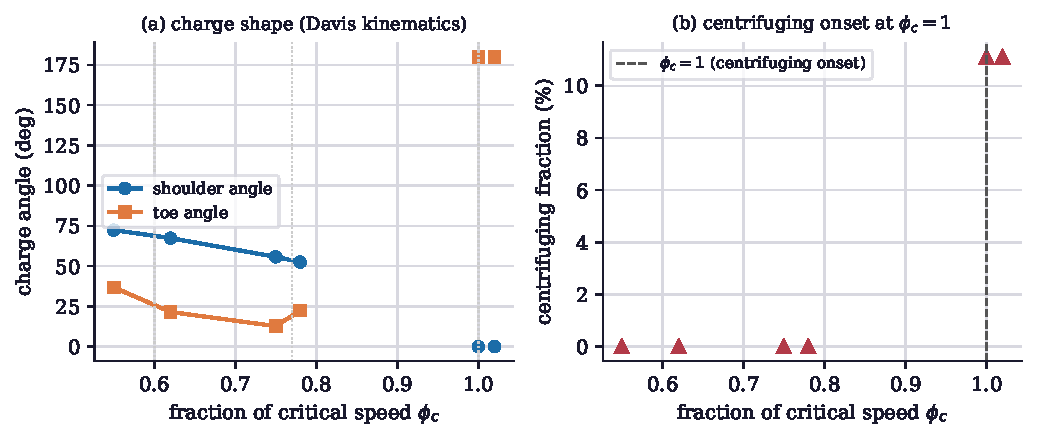
\includegraphics[width=0.84\textwidth]{fig-regimes.pdf}
\caption{Charge motion by Davis kinematics, across ten cases. \textbf{(a)} The shoulder and toe angles against
the fraction of critical speed $\phi_c$: as $\phi_c$ rises the charge lifts higher (the shoulder rises, the toe
advances) through the cascading and cataracting regimes, and at the critical speed the charge centrifuges (the
shoulder collapses to zero and the toe to $180^\circ$, the charge pinned to the shell). \textbf{(b)} The
centrifuging fraction is zero below the critical speed and turns on exactly at $\phi_c=1$, the exact onset Davis
kinematics predicts.}
\label{fig:regimes}
\end{figure*}

\section{Charge Motion: Davis Kinematics}\label{sec:motion}

The charge shape and regime follow from Davis kinematics evaluated over nine radial shells
(Fig.~\ref{fig:regimes}). As the fraction of critical speed rises, the charge is carried higher before it departs,
so the shoulder angle rises and the toe advances, and the motion passes through the literature regime bands:
slumping and cascading at low speed (here $\phi_c\approx0.55$--$0.62$, shoulder near $70^\circ$), cataracting at
intermediate speed ($\phi_c\approx0.75$--$0.78$, the ballistic fan that does the impact grinding in a SAG mill),
and centrifuging at the critical speed. The centrifuging onset is exact: below $\phi_c=1$ no shell centrifuges,
and at $\phi_c=1$ the outer shell pins to the wall, the shoulder collapses to zero and the toe to $180^\circ$
(Fig.~\ref{fig:regimes}b). Because the critical speed and $\phi_c$ are derived from geometry, not fitted, the
regime map is a property of the kinematics, and it reproduces the textbook picture, which is the check that
licenses using the workbench to reason about charge motion.

\section{Power: Where the Standard Models Disagree}\label{sec:power}

\begin{figure*}[!t]
\centering
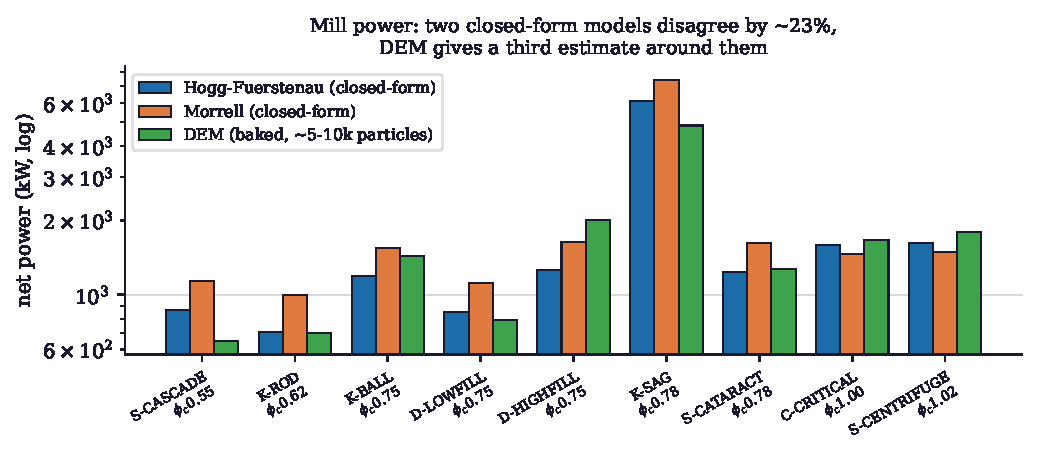
\includegraphics[width=0.84\textwidth]{fig-power.pdf}
\caption{Net mill power per case, on a log axis, from two closed-form models and from a baked discrete-element
simulation. The Hogg-Fuerstenau and Morrell closed-form models \emph{disagree by about $23\%$} (median; up to
$29\%$): Morrell is consistently higher at cascading and cataracting speeds, and the two cross near the critical
speed. The discrete-element estimate ($5000$--$10000$ particles) lands around them, sometimes below both, sometimes
above, rather than settling the disagreement. This spread is the cross-method uncertainty of mill-power
prediction, and the workbench shows all three rather than reporting one as fact.}
\label{fig:power}
\end{figure*}

The power is where the comparison between models matters most (Fig.~\ref{fig:power}, Table~\ref{tab:power}).
Two standard closed-form models are computed: Hogg-Fuerstenau~\cite{hogg}, a torque-arm model with an
effective-lift-arm calibration ($C_{\text{arm}}=0.80$, stated in the interface), and Morrell~\cite{morrell}. They
do not agree. Across the ten cases the two disagree by a median of $23\%$ and by as much as $29\%$: Morrell draws
consistently higher at the cascading and cataracting speeds that mills actually run at (for example
$1139$~kW against $872$~kW on a cascading case), and the two only cross near the critical speed. A third estimate,
from a baked discrete-element simulation of five to ten thousand particles, lands \emph{around} the two closed-form
values, below both on some cases and above on others, rather than adjudicating between them. The spread is a
property of the models, not of the workbench: on these cases the two standard models differ by 18 to 29 percent
below the critical speed, so a single power reported to four significant figures would assert a precision that
the models do not support. ChargeCascade shows the two closed-form models and the discrete-element estimate together, with the
Hogg-Fuerstenau calibration stated, so a user sees the spread and can reason about it.

\begin{table}[!t]
\centering
\caption{Net power by the two closed-form models and the baked DEM for six representative cases of the ten; the
empty-mill case \texttt{C-EMPTY}, whose closed-form power is zero, is omitted. Below the critical speed the
closed-form models disagree by 18--29\% of the larger value, and they cross near it (8\% at \texttt{C-CRITICAL});
DEM lands around them.}
\label{tab:power}
\footnotesize
\begin{tabular}{@{}l c r r r@{}}
\toprule
Case & $\phi_c$ & Hogg-F. (kW) & Morrell (kW) & DEM (kW) \\
\midrule
S-CASCADE   & $0.55$ & $872$  & $1139$ & $649$  \\
K-ROD       & $0.62$ & $704$  & $995$  & $699$  \\
K-BALL      & $0.75$ & $1188$ & $1553$ & $1435$ \\
D-HIGHFILL  & $0.75$ & $1256$ & $1642$ & $2005$ \\
K-SAG       & $0.78$ & $6111$ & $7440$ & $4852$ \\
C-CRITICAL  & $1.00$ & $1584$ & $1464$ & $1667$ \\
\bottomrule
\end{tabular}
\end{table}

\section{The Learned Surrogate and Its Guard}\label{sec:surrogate}

For instant what-if exploration the workbench runs a learned surrogate of the closed-form engine: a small
multilayer perceptron (six inputs, two hidden layers of sixty-four units, mapping to power and centrifuging
fraction) trained on the engine's outputs. It reproduces the closed-form power to a mean relative error of
$5.2\%$ (with the centrifuging fraction exactly, since it is a kinematic threshold), fast enough to update as a
user drags a control. Crucially, because a surrogate is only reliable inside the envelope it was trained on, a
companion out-of-distribution detector flags settings outside that envelope, so a user who pushes the sliders to
an untrained corner is warned that the surrogate is extrapolating rather than being silently misled. A learned
DEM surrogate, a graph-network simulator trained to roll the particle dynamics forward, is under development; it
is not validated, and no result reported here uses it. The surrogate accelerates the engine; the underlying model
disagreement remains displayed beside it.

\section{Discussion and Scope}\label{sec:discuss}

The workbench's contribution is as much epistemic as computational: it computes tumbling-mill charge motion and
power from the cited models and, by showing the Hogg-Fuerstenau and Morrell models and the discrete-element
estimate together, it makes the cross-method uncertainty of mill-power prediction visible. The
Hogg-Fuerstenau effective-lift-arm calibration is a stated constant, not a fit to a specific mill, and the
interface shows it; the Morrell model is used as published. The cases are physically reasonable
synthetic configurations, not a specific plant, so the numbers are the models' behaviour, not a prediction for a
given mill. The baked discrete-element traces are a higher-fidelity but still-modelled estimate at laboratory
particle counts, not a measured power, and the graph-network DEM surrogate is still under development. The value
is a reproducible workbench that presents mill-power prediction together with its cross-method spread. The
interface states the same limits on its methodology pages.

\section{Conclusion}

ChargeCascade computes tumbling-mill charge motion by Davis kinematics, reproducing the cascading-cataracting-%
centrifuging progression with an exact centrifuging onset at the critical speed, and computes the power by two
standard closed-form models plus a baked discrete-element estimate. Its central finding is that the two
textbook power models disagree by about a fifth, and it displays that spread with the third estimate around it,
rather than reporting one number as fact, because a fifth is the cross-method uncertainty between these models. A
learned surrogate reproduces the closed-form power to $5.2\%$ with an out-of-distribution guard. The
contribution is a reproducible workbench that displays the model disagreement and states its one calibration
constant.

\appendices
\section{Reproduction}\label{app:repro}

The repository artifacts under \path{data/derived/} carry the ten cases' engine outputs
(\path{case-results.json}: $\phi_c$, regime, shoulder and toe angles, centrifuging fraction, and both the
Hogg-Fuerstenau and Morrell power per case), the learned-surrogate metrics (\path{cc-learned.json}) and the
baked DEM summaries (\path{data/dem/}). The figure scripts under
\path{manuscripts/mill-charge-power/figures/} read those artifacts. The same dependency-free physics engine
serves the interactive workbench, the experiment tables and the offline bake, so re-running reproduces
Table~\ref{tab:power} and Figs.~\ref{fig:regimes}--\ref{fig:power}.

\balance

\begin{thebibliography}{00}

\bibitem{davis} E.~W. Davis, ``Fine crushing in ball-mills,'' \emph{Transactions of the American Institute of
Mining Engineers}, vol.~61, pp.~250--296, 1919.

\bibitem{hogg} R.~Hogg and D.~W. Fuerstenau, ``Power relations for tumbling mills,'' \emph{Transactions
SME-AIME}, vol.~252, pp.~418--423, 1972.

\bibitem{morrell} S.~Morrell, \emph{The Prediction of Power Draw in Wet Tumbling Mills}, Ph.D. dissertation,
University of Queensland (JKMRC), Brisbane, Australia, 1993. doi:10.14264/252760.

\bibitem{mishra} B.~K. Mishra and R.~K. Rajamani, ``The discrete element method for the simulation of ball
mills,'' \emph{Applied Mathematical Modelling}, vol.~16, no.~11, pp.~598--604, 1992.
doi:10.1016/0307-904X(92)90035-2.

\bibitem{cleary98} P.~W. Cleary, ``Predicting charge motion, power draw, segregation and wear in ball mills using
discrete element methods,'' \emph{Minerals Engineering}, vol.~11, no.~11, pp.~1061--1080, 1998.
doi:10.1016/S0892-6875(98)00093-4.

\bibitem{cleary01} P.~W. Cleary, ``Charge behaviour and power consumption in ball mills: sensitivity to mill
operating conditions, liner geometry and charge composition,'' \emph{International Journal of Mineral
Processing}, vol.~63, no.~2, pp.~79--114, 2001. doi:10.1016/S0301-7516(01)00037-0.

\end{thebibliography}

\end{document}
